% Generated by LitigCharts.PublicationFigures. Captions and provenance are sidecars.
\documentclass[10pt,tikz,border=5pt]{standalone}
\usepackage{lmodern}
\usetikzlibrary{patterns,patterns.meta}
\begin{document}
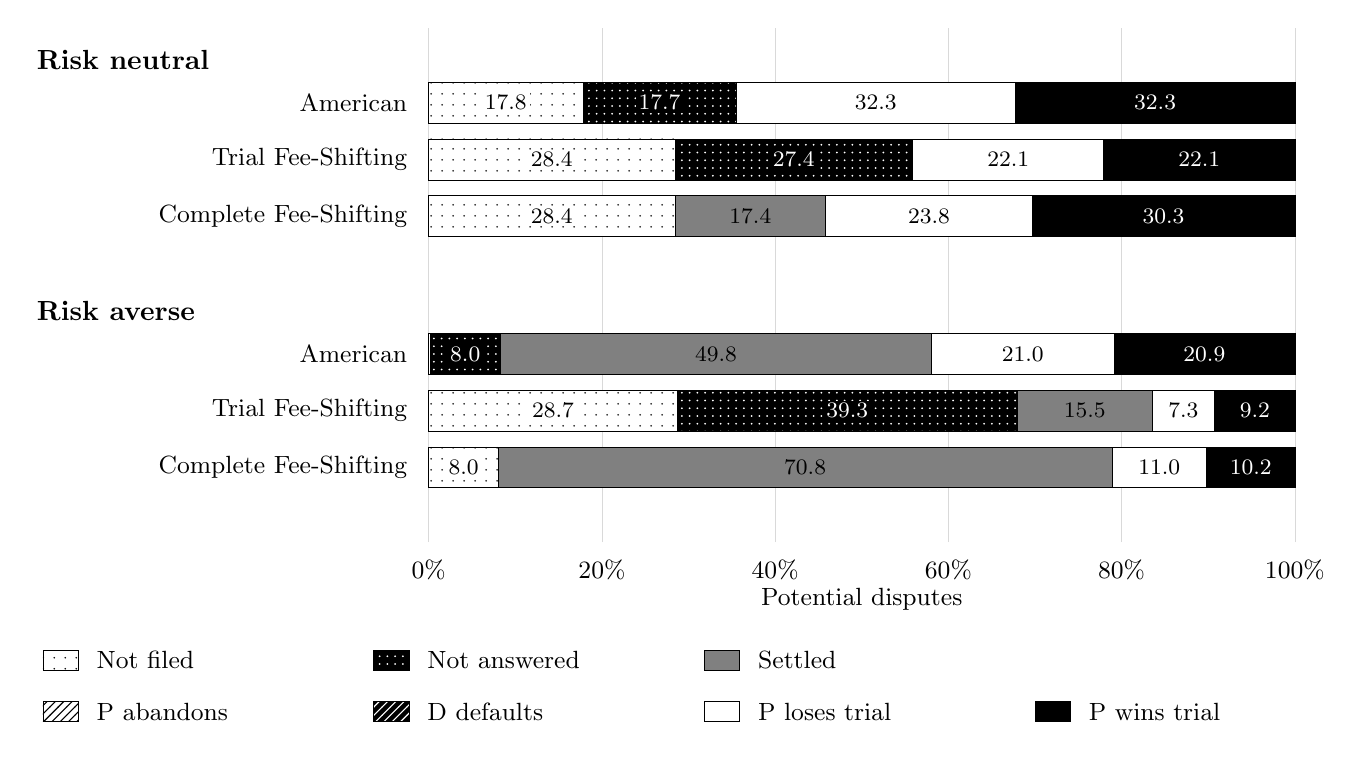
\begin{tikzpicture}[font=\small]\draw[black!15,line width=.2pt] (5.1,.65) -- (5.1,7.18);
\node[anchor=north] at (5.1,.55) {0\%};
\draw[black!15,line width=.2pt] (7.3,.65) -- (7.3,7.18);
\node[anchor=north] at (7.3,.55) {20\%};
\draw[black!15,line width=.2pt] (9.5,.65) -- (9.5,7.18);
\node[anchor=north] at (9.5,.55) {40\%};
\draw[black!15,line width=.2pt] (11.7,.65) -- (11.7,7.18);
\node[anchor=north] at (11.7,.55) {60\%};
\draw[black!15,line width=.2pt] (13.9,.65) -- (13.9,7.18);
\node[anchor=north] at (13.9,.55) {80\%};
\draw[black!15,line width=.2pt] (16.1,.65) -- (16.1,7.18);
\node[anchor=north] at (16.1,.55) {100\%};
\node[anchor=west,font=\bfseries] at (0,6.78) {\mbox{Risk} \mbox{neutral}};
\node[anchor=east] at (4.95,6.23) {American};
\path[preaction={fill=white,draw=none},pattern={Dots[distance=4pt,radius=.35pt]},pattern color=black,draw=black,line width=.25pt] (5.1,5.97) rectangle (7.05943,6.49);
\node[text=black,fill=white,font=\footnotesize,inner sep=1pt] at (6.079715,6.23) {17.8};
\path[preaction={fill=black,draw=none},pattern={Dots[distance=2.8pt,radius=.35pt]},pattern color=white,draw=black,line width=.25pt] (7.05943,5.97) rectangle (9.002382,6.49);
\node[text=white,fill=black,font=\footnotesize,inner sep=1pt] at (8.030906,6.23) {17.7};
\path[fill=white,draw=black,line width=.25pt] (9.002382,5.97) rectangle (12.551235,6.49);
\node[text=black,fill=none,font=\footnotesize,inner sep=1pt] at (10.776809,6.23) {32.3};
\path[fill=black,draw=black,line width=.25pt] (12.551235,5.97) rectangle (16.1,6.49);
\node[text=white,fill=none,font=\footnotesize,inner sep=1pt] at (14.325618,6.23) {32.3};
\node[anchor=east] at (4.95,5.51) {Trial Fee-Shifting};
\path[preaction={fill=white,draw=none},pattern={Dots[distance=4pt,radius=.35pt]},pattern color=black,draw=black,line width=.25pt] (5.1,5.25) rectangle (8.22741,5.77);
\node[text=black,fill=white,font=\footnotesize,inner sep=1pt] at (6.663705,5.51) {28.4};
\path[preaction={fill=black,draw=none},pattern={Dots[distance=2.8pt,radius=.35pt]},pattern color=white,draw=black,line width=.25pt] (8.22741,5.25) rectangle (11.246525,5.77);
\node[text=white,fill=black,font=\footnotesize,inner sep=1pt] at (9.736968,5.51) {27.4};
\path[fill=white,draw=black,line width=.25pt] (11.246525,5.25) rectangle (13.67329,5.77);
\node[text=black,fill=none,font=\footnotesize,inner sep=1pt] at (12.459908,5.51) {22.1};
\path[fill=black,draw=black,line width=.25pt] (13.67329,5.25) rectangle (16.1,5.77);
\node[text=white,fill=none,font=\footnotesize,inner sep=1pt] at (14.886645,5.51) {22.1};
\node[anchor=east] at (4.95,4.79) {Complete Fee-Shifting};
\path[preaction={fill=white,draw=none},pattern={Dots[distance=4pt,radius=.35pt]},pattern color=black,draw=black,line width=.25pt] (5.1,4.53) rectangle (8.22741,5.05);
\node[text=black,fill=white,font=\footnotesize,inner sep=1pt] at (6.663705,4.79) {28.4};
\path[fill=black!50,draw=black,line width=.25pt] (8.22741,4.53) rectangle (10.142741,5.05);
\node[text=black,fill=none,font=\footnotesize,inner sep=1pt] at (9.185076,4.79) {17.4};
\path[fill=white,draw=black,line width=.25pt] (10.142741,4.53) rectangle (12.764151,5.05);
\node[text=black,fill=none,font=\footnotesize,inner sep=1pt] at (11.453446,4.79) {23.8};
\path[fill=black,draw=black,line width=.25pt] (12.764151,4.53) rectangle (16.1,5.05);
\node[text=white,fill=none,font=\footnotesize,inner sep=1pt] at (14.432076,4.79) {30.3};
\node[anchor=west,font=\bfseries] at (0,3.59) {\mbox{Risk} \mbox{averse}};
\node[anchor=east] at (4.95,3.04) {American};
\path[preaction={fill=white,draw=none},pattern={Dots[distance=4pt,radius=.35pt]},pattern color=black,draw=black,line width=.25pt] (5.1,2.78) rectangle (5.121903,3.3);
\path[preaction={fill=black,draw=none},pattern={Dots[distance=2.8pt,radius=.35pt]},pattern color=white,draw=black,line width=.25pt] (5.121903,2.78) rectangle (6.006797,3.3);
\node[text=white,fill=black,font=\footnotesize,inner sep=1pt] at (5.56435,3.04) {8.0};
\path[fill=black!50,draw=black,line width=.25pt] (6.006797,2.78) rectangle (11.488889,3.3);
\node[text=black,fill=none,font=\footnotesize,inner sep=1pt] at (8.747843,3.04) {49.8};
\path[fill=white,draw=black,line width=.25pt] (11.488889,2.78) rectangle (13.802255,3.3);
\node[text=black,fill=none,font=\footnotesize,inner sep=1pt] at (12.645572,3.04) {21.0};
\path[fill=black,draw=black,line width=.25pt] (13.802255,2.78) rectangle (16.100001,3.3);
\node[text=white,fill=none,font=\footnotesize,inner sep=1pt] at (14.951128,3.04) {20.9};
\node[anchor=east] at (4.95,2.32) {Trial Fee-Shifting};
\path[preaction={fill=white,draw=none},pattern={Dots[distance=4pt,radius=.35pt]},pattern color=black,draw=black,line width=.25pt] (5.1,2.06) rectangle (8.255152,2.58);
\node[text=black,fill=white,font=\footnotesize,inner sep=1pt] at (6.677576,2.32) {28.7};
\path[preaction={fill=black,draw=none},pattern={Dots[distance=2.8pt,radius=.35pt]},pattern color=white,draw=black,line width=.25pt] (8.255152,2.06) rectangle (12.576392,2.58);
\node[text=white,fill=black,font=\footnotesize,inner sep=1pt] at (10.415772,2.32) {39.3};
\path[fill=black!50,draw=black,line width=.25pt] (12.576392,2.06) rectangle (14.286045,2.58);
\node[text=black,fill=none,font=\footnotesize,inner sep=1pt] at (13.431219,2.32) {15.5};
\path[fill=white,draw=black,line width=.25pt] (14.286045,2.06) rectangle (15.083881,2.58);
\node[text=black,fill=none,font=\footnotesize,inner sep=1pt] at (14.684963,2.32) {7.3};
\path[fill=black,draw=black,line width=.25pt] (15.083881,2.06) rectangle (16.099999,2.58);
\node[text=white,fill=none,font=\footnotesize,inner sep=1pt] at (15.59194,2.32) {9.2};
\node[anchor=east] at (4.95,1.6) {Complete Fee-Shifting};
\path[preaction={fill=white,draw=none},pattern={Dots[distance=4pt,radius=.35pt]},pattern color=black,draw=black,line width=.25pt] (5.1,1.34) rectangle (5.98495,1.86);
\node[text=black,fill=white,font=\footnotesize,inner sep=1pt] at (5.542475,1.6) {8.0};
\path[fill=black!50,draw=black,line width=.25pt] (5.98495,1.34) rectangle (13.77592,1.86);
\node[text=black,fill=none,font=\footnotesize,inner sep=1pt] at (9.880435,1.6) {70.8};
\path[fill=white,draw=black,line width=.25pt] (13.77592,1.34) rectangle (14.981179,1.86);
\node[text=black,fill=none,font=\footnotesize,inner sep=1pt] at (14.37855,1.6) {11.0};
\path[fill=black,draw=black,line width=.25pt] (14.981179,1.34) rectangle (16.1,1.86);
\node[text=white,fill=none,font=\footnotesize,inner sep=1pt] at (15.54059,1.6) {10.2};
\node at (10.6,-.08) {Potential disputes};
\path[preaction={fill=white,draw=none},pattern={Dots[distance=4pt,radius=.35pt]},pattern color=black,draw=black,line width=.25pt] (0.2,-0.98) rectangle (0.65,-0.72);
\node[anchor=west] at (0.76,-0.85) {Not filed};
\path[preaction={fill=black,draw=none},pattern={Dots[distance=2.8pt,radius=.35pt]},pattern color=white,draw=black,line width=.25pt] (4.4,-0.98) rectangle (4.85,-0.72);
\node[anchor=west] at (4.96,-0.85) {Not answered};
\path[fill=black!50,draw=black,line width=.25pt] (8.6,-0.98) rectangle (9.05,-0.72);
\node[anchor=west] at (9.16,-0.85) {Settled};
\path[preaction={fill=white,draw=none},pattern={north east lines},pattern color=black,draw=black,line width=.25pt] (0.2,-1.63) rectangle (0.65,-1.37);
\node[anchor=west] at (0.76,-1.5) {P abandons};
\path[preaction={fill=black,draw=none},pattern={north east lines},pattern color=white,draw=black,line width=.25pt] (4.4,-1.63) rectangle (4.85,-1.37);
\node[anchor=west] at (4.96,-1.5) {D defaults};
\path[fill=white,draw=black,line width=.25pt] (8.6,-1.63) rectangle (9.05,-1.37);
\node[anchor=west] at (9.16,-1.5) {P loses trial};
\path[fill=black,draw=black,line width=.25pt] (12.8,-1.63) rectangle (13.25,-1.37);
\node[anchor=west] at (13.36,-1.5) {P wins trial};
\end{tikzpicture}
\end{document}
